\section{ Experiments and Results} \label{experiment}
For our experiments, we ran our data one NVIDIA Tesla K80 GPU available on Google Cloud using CUDA 9.0 and PyTorch 0.4, along with a local Pascal GTX 1080 GPU using CUDA 10.0 and PyTorch 1.0. We used 1056 images of size $256 \times 256$ as for training, and 452 images for testing. The training phase takes about 11 hours to finish if the complete training dataset is used.

\begin{figure*}[h]
	\def\tabularxcolumn#1{m{#1}}

	\begin{tabularx}{\linewidth}{| c | c | c |}
	
		\begin{tabular}{cc}
			\subfloat{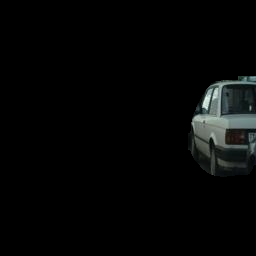
\includegraphics[width=2.7cm, height=2.7cm]{./figure/126_real_B}}\\ 
			ground truth \\
		\end{tabular}
		&
		\begin{tabular}{cc}
			\subfloat{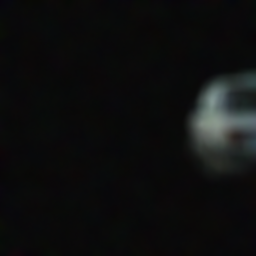
\includegraphics[width=2.7cm, height=2.7cm]{./figure/126_real_A}}\\  
			blurred image\\
		\end{tabular}
		&
		\begin{tabular}{cc}
			\subfloat{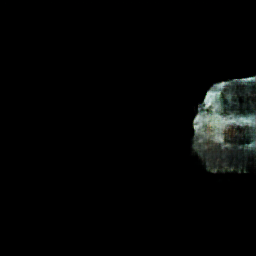
\includegraphics[width=2.7cm, height=2.7cm]{./figure/126_fake_B}}\\ 
			generated image \\
		\end{tabular}
	\end{tabularx}	
	\caption{Result from the first experiment. The GAN has succesfully estimated the boundary of the car.}\label{fig1}
\end{figure*}

The first experiment we ran was using blurred images as input. We took the images of cars, added some Gaussian noise and convolved the image with a two-dimensional $sinc$ function. We fed these images as input, and the original images to the network as ground truth. the results showed that the network is able to restore the boundaries of the cars with a high accuracy. The problem with this implementation was that the image was not gray-scaled, and we did not go through a precise simulation according the to underlying physics of mmWave radars to generate the images. The purpose of this step was to evaluate the feasibility of our idea of restoring the boundaries using GANs on a high level. The results from this experiments are shown in figure \ref{fig1}. It can be seen that the boundary of the car has been fairly accurately reconstructed. It is also noteworthy that the GAN was able to restore the side mirror of the car successfully, although there is no side mirror visible point in GAN. 

\begin{figure*}
	\def\tabularxcolumn#1{m{#1}}
	\begin{tabularx}{\linewidth}{| c | c | c | c | c | }
		\begin{tabular}{cc}
			\subfloat{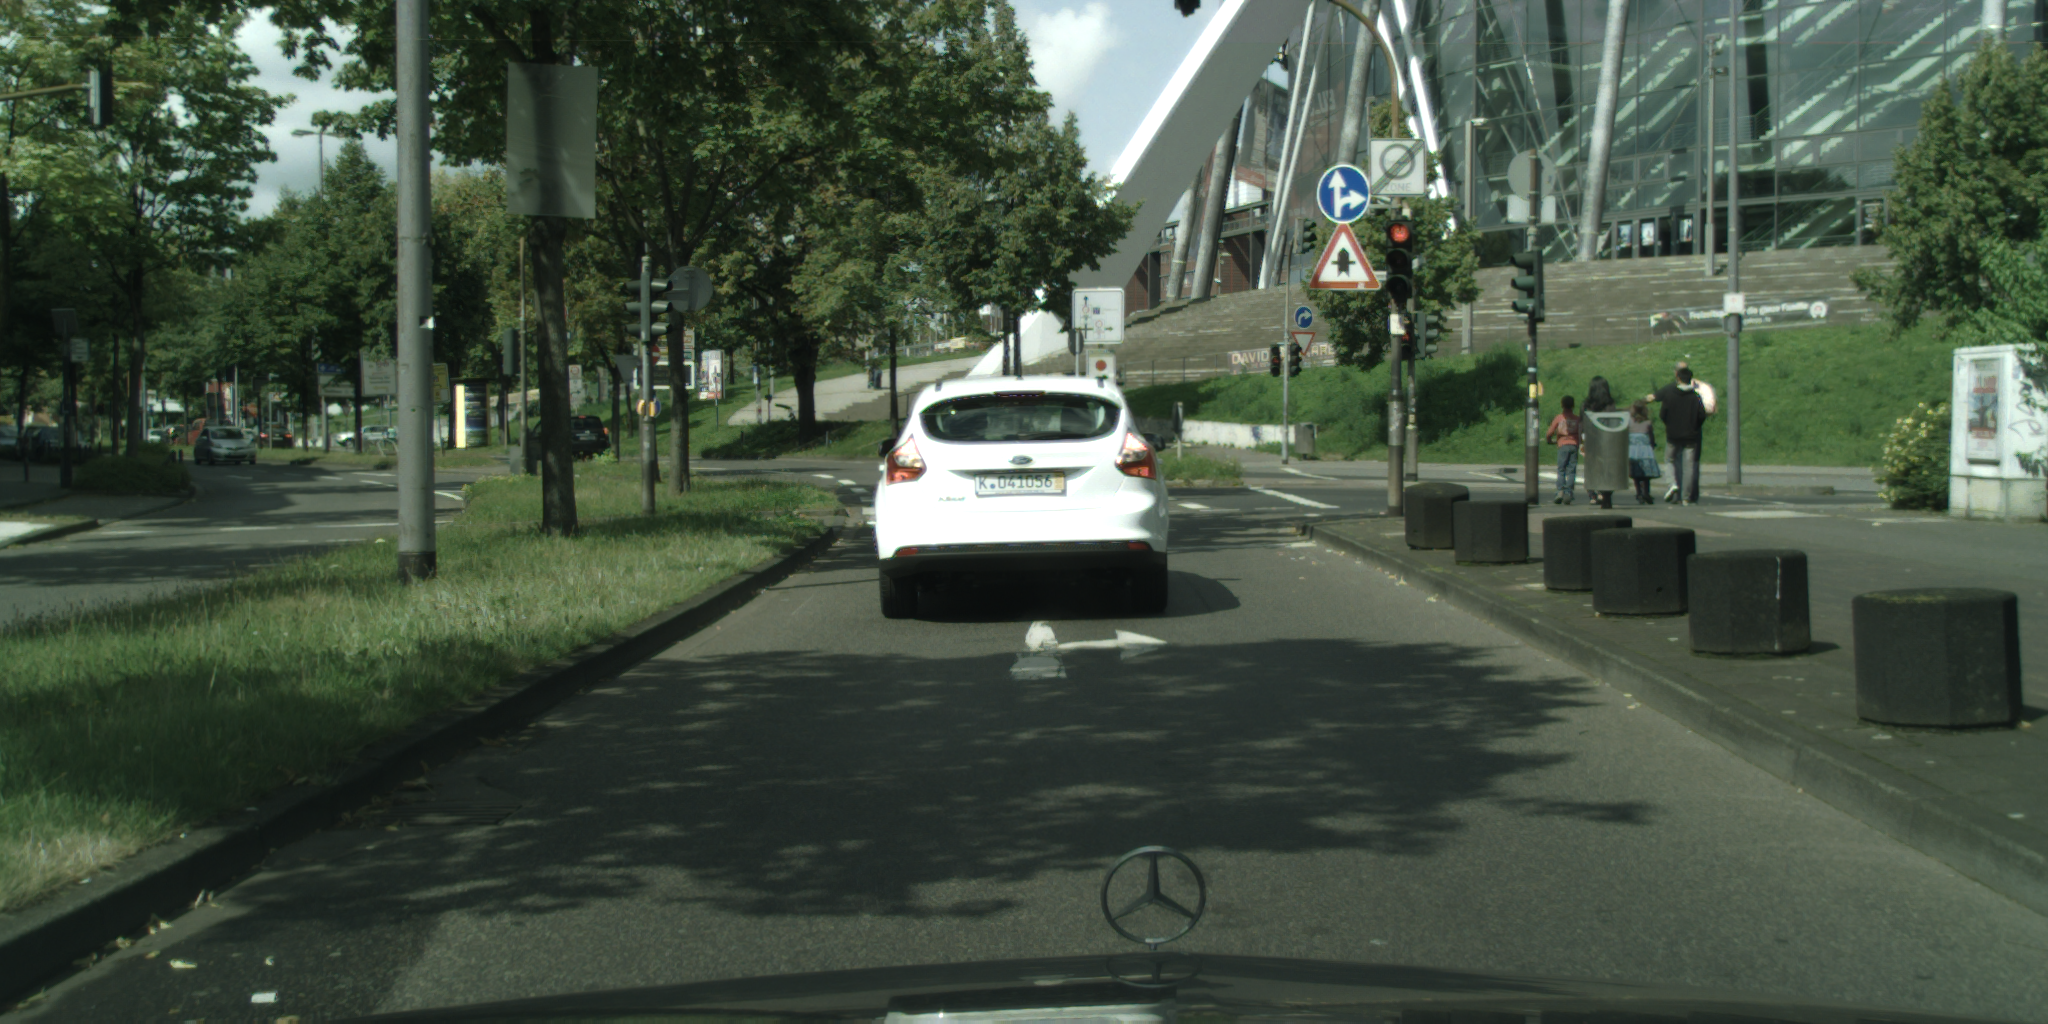
\includegraphics[width=2.7cm, height=2.7cm]{./figure/cologne_000011_000019_leftImg8bit}}\\ 
			\subfloat{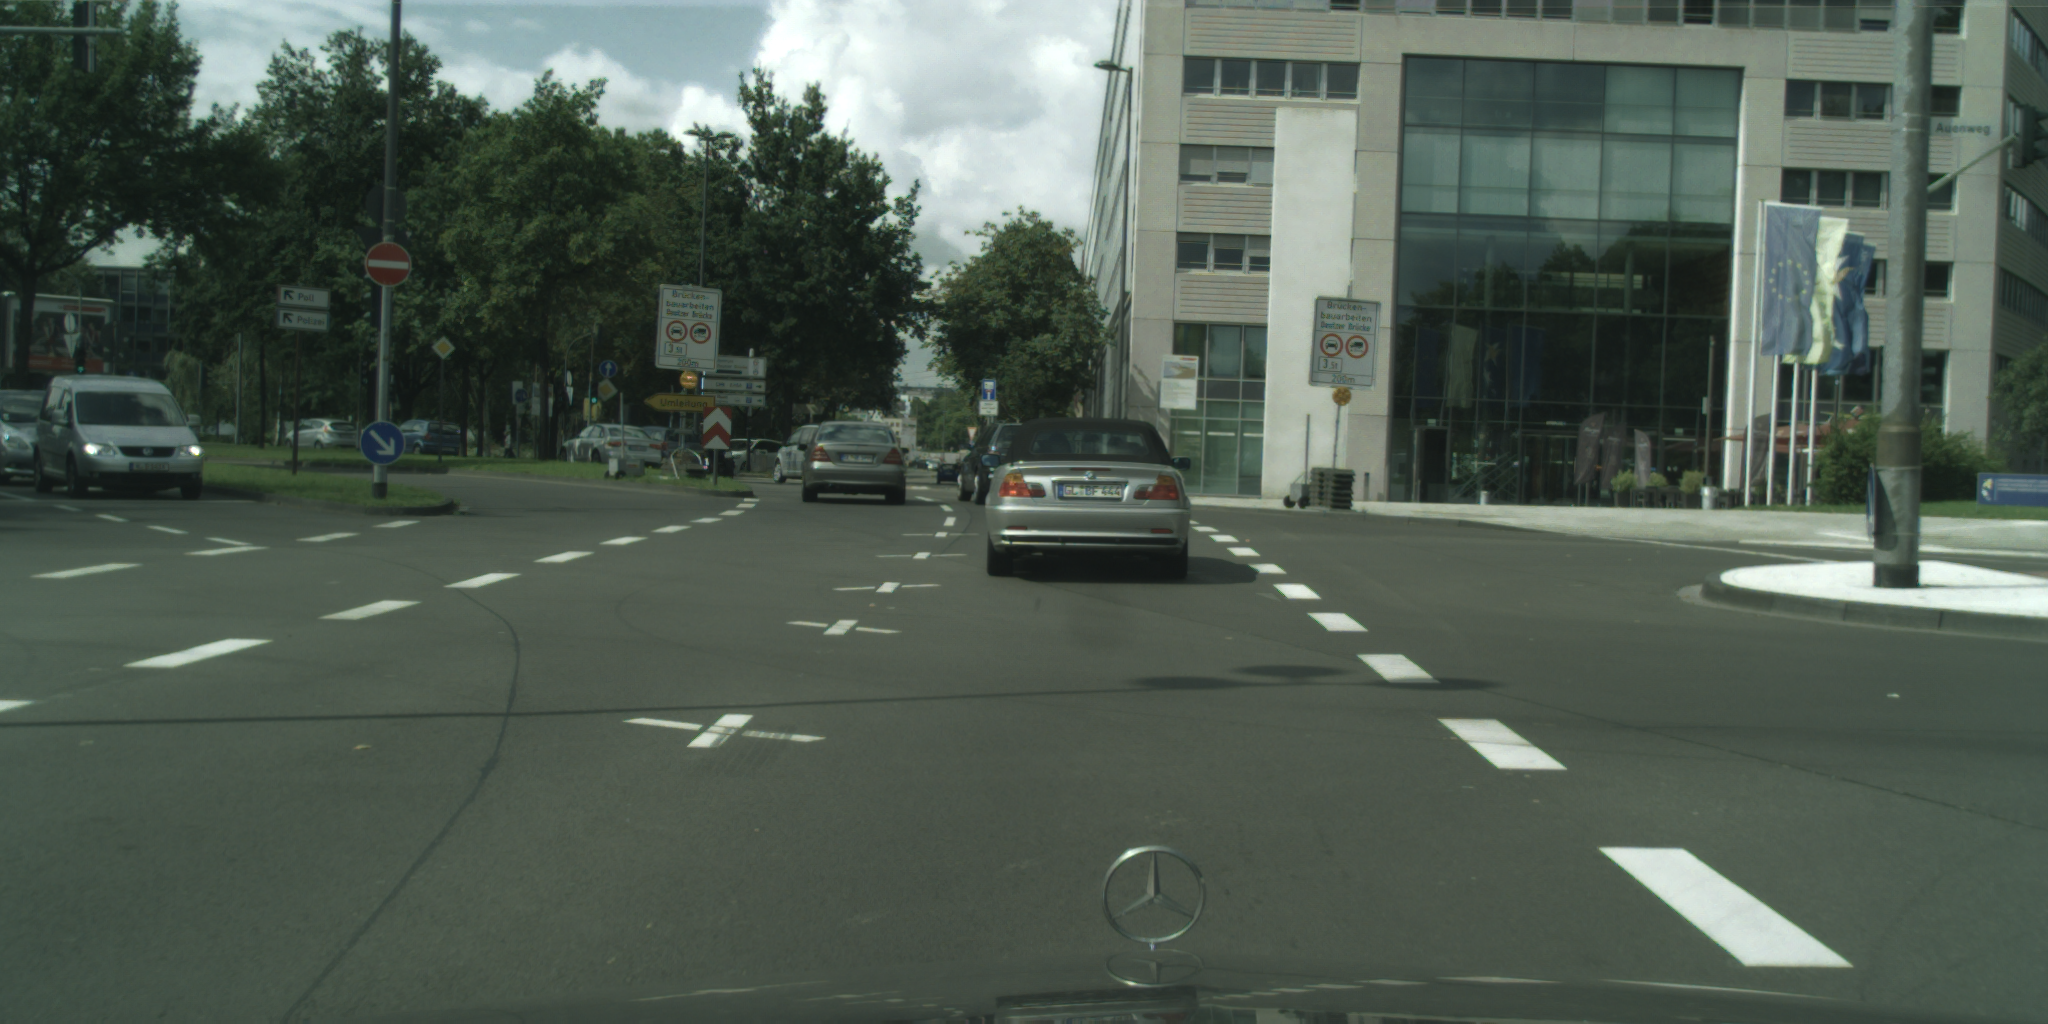
\includegraphics[width=2.7cm, height=2.7cm]{./figure/cologne_000013_000019_leftImg8bit.png}}\\
			\subfloat{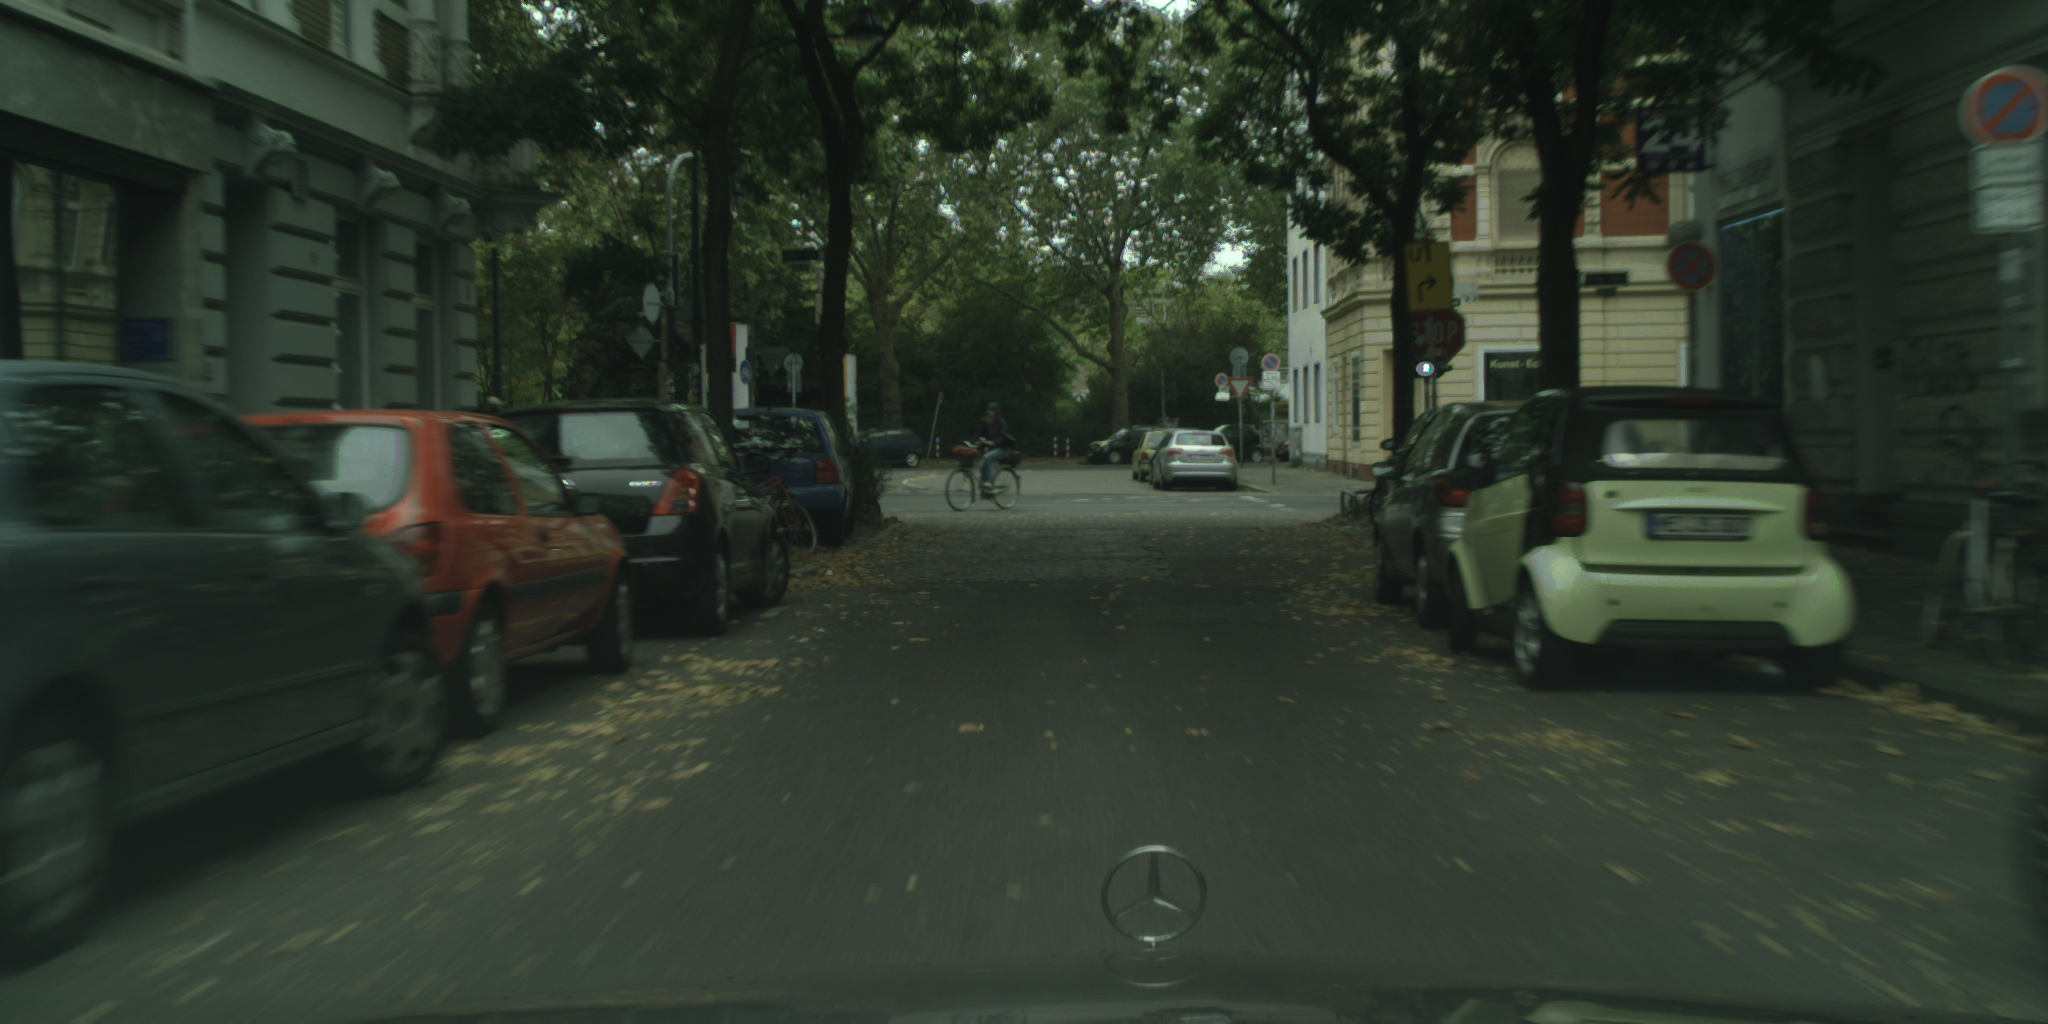
\includegraphics[width=2.7cm, height=2.7cm]{./figure/dusseldorf_000008_000019_leftImg8bit.png}}\\ 
			\subfloat{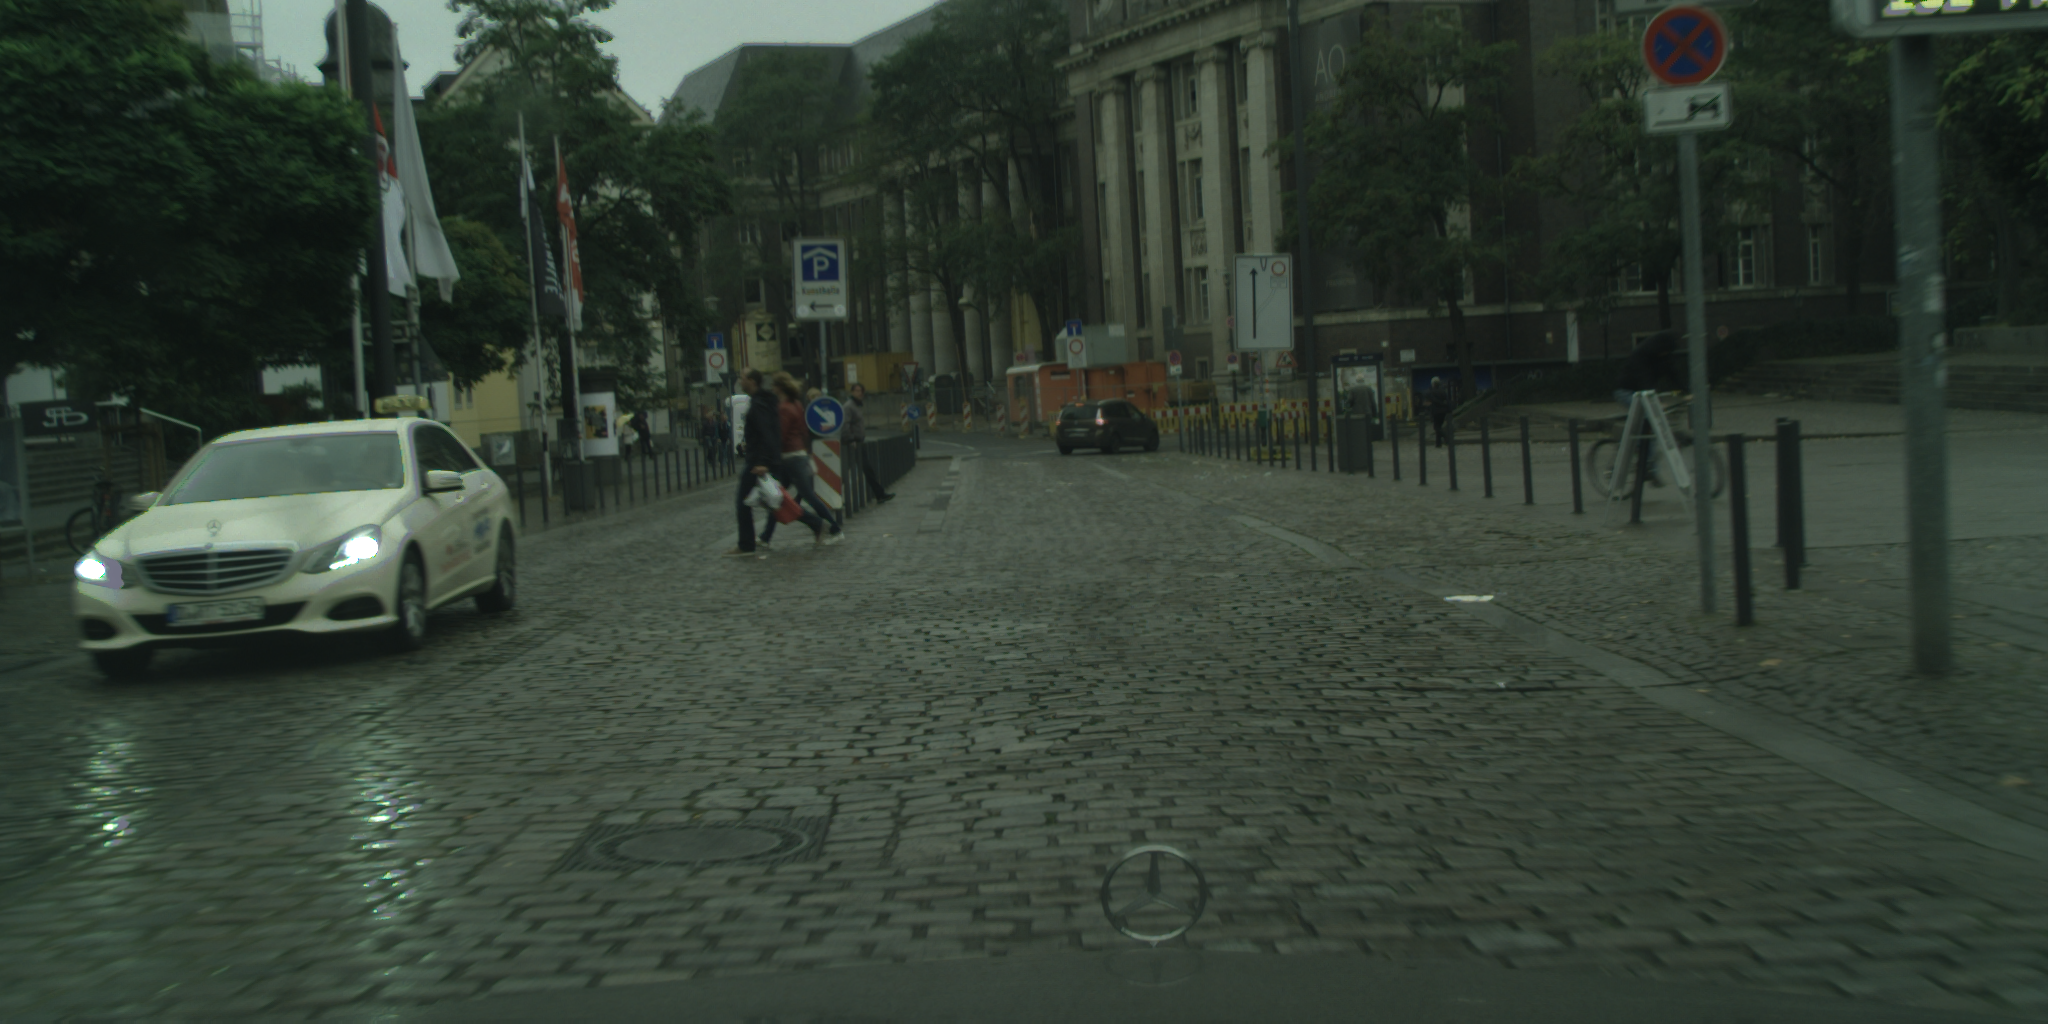
\includegraphics[width=2.7cm, height=2.7cm]{./figure/dusseldorf_000040_000019_leftImg8bit.png}}\\
			\subfloat{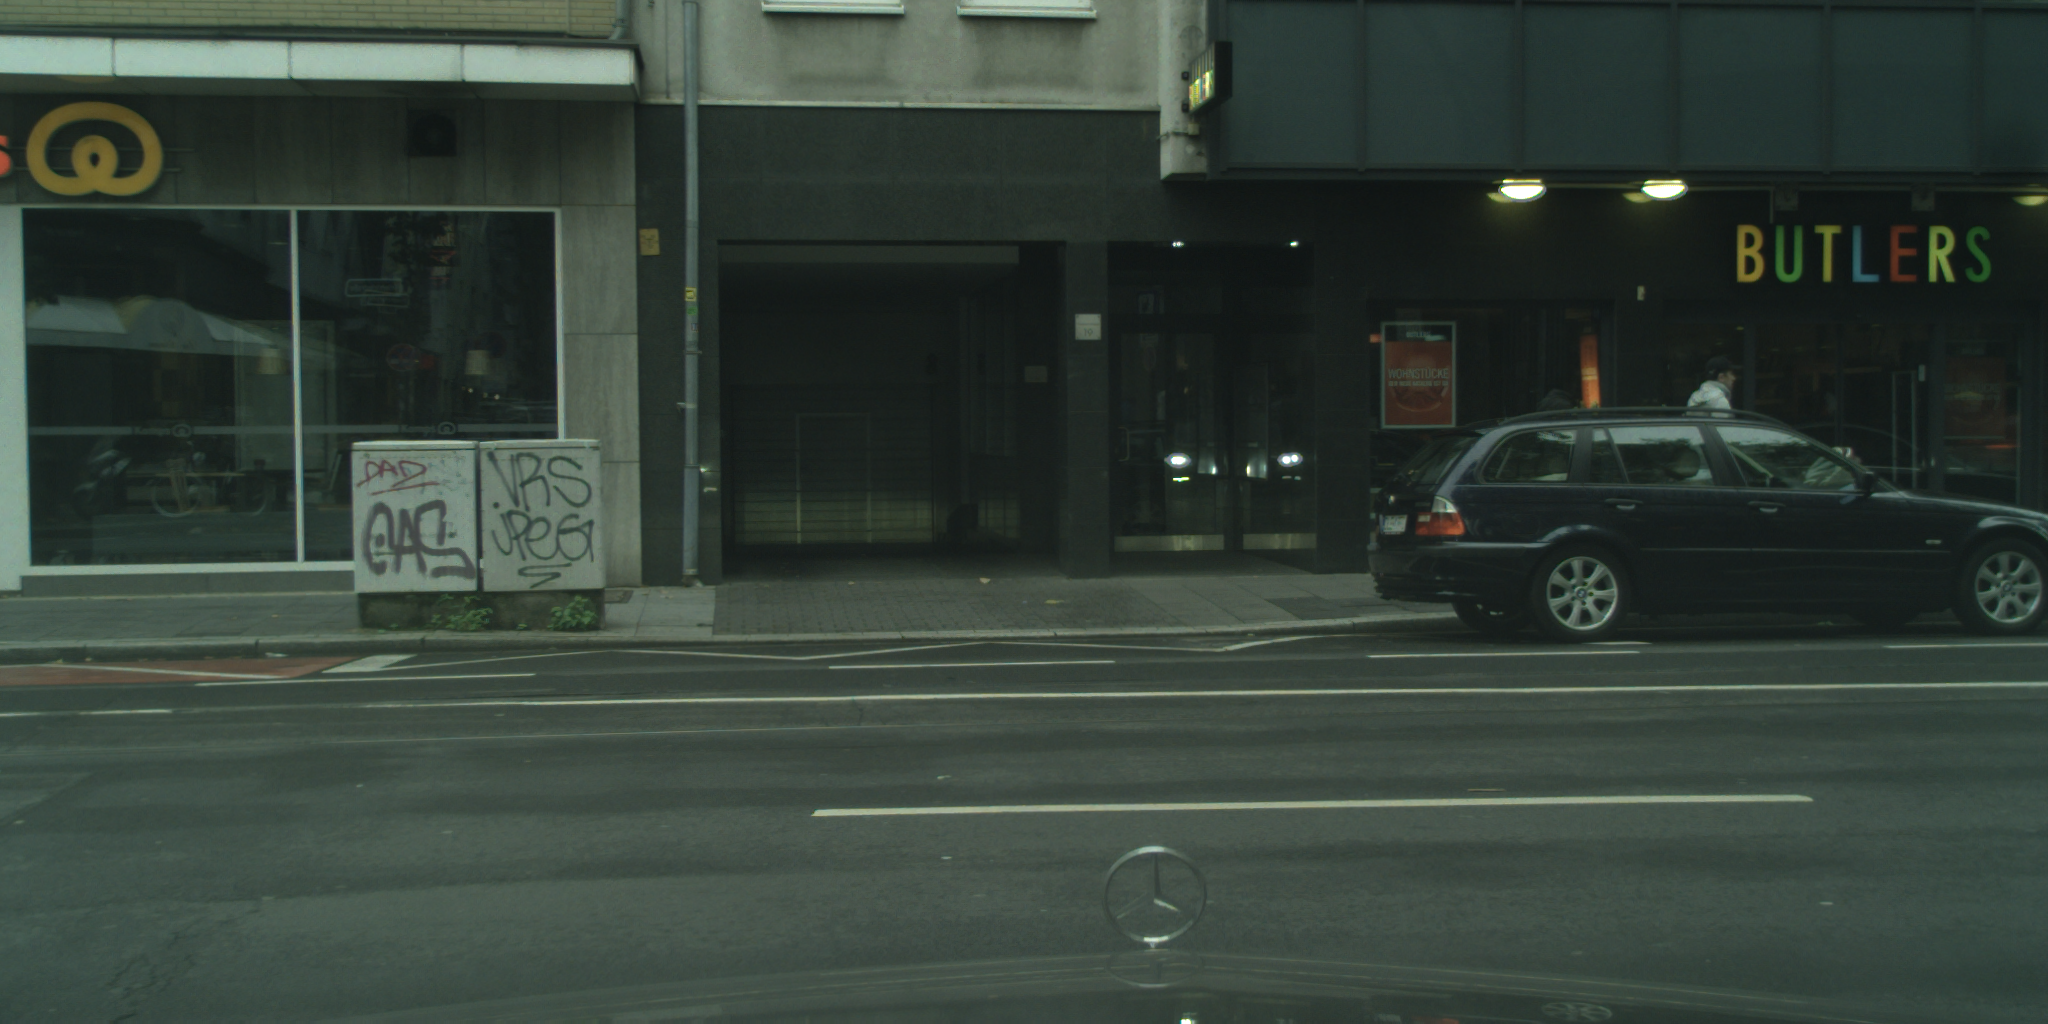
\includegraphics[width=2.7cm, height=2.7cm]{./figure/dusseldorf_000088_000019_leftImg8bit.png}}\\ 
			(a) original image \\
		\end{tabular}
		&
		\begin{tabular}{cc}
			\subfloat{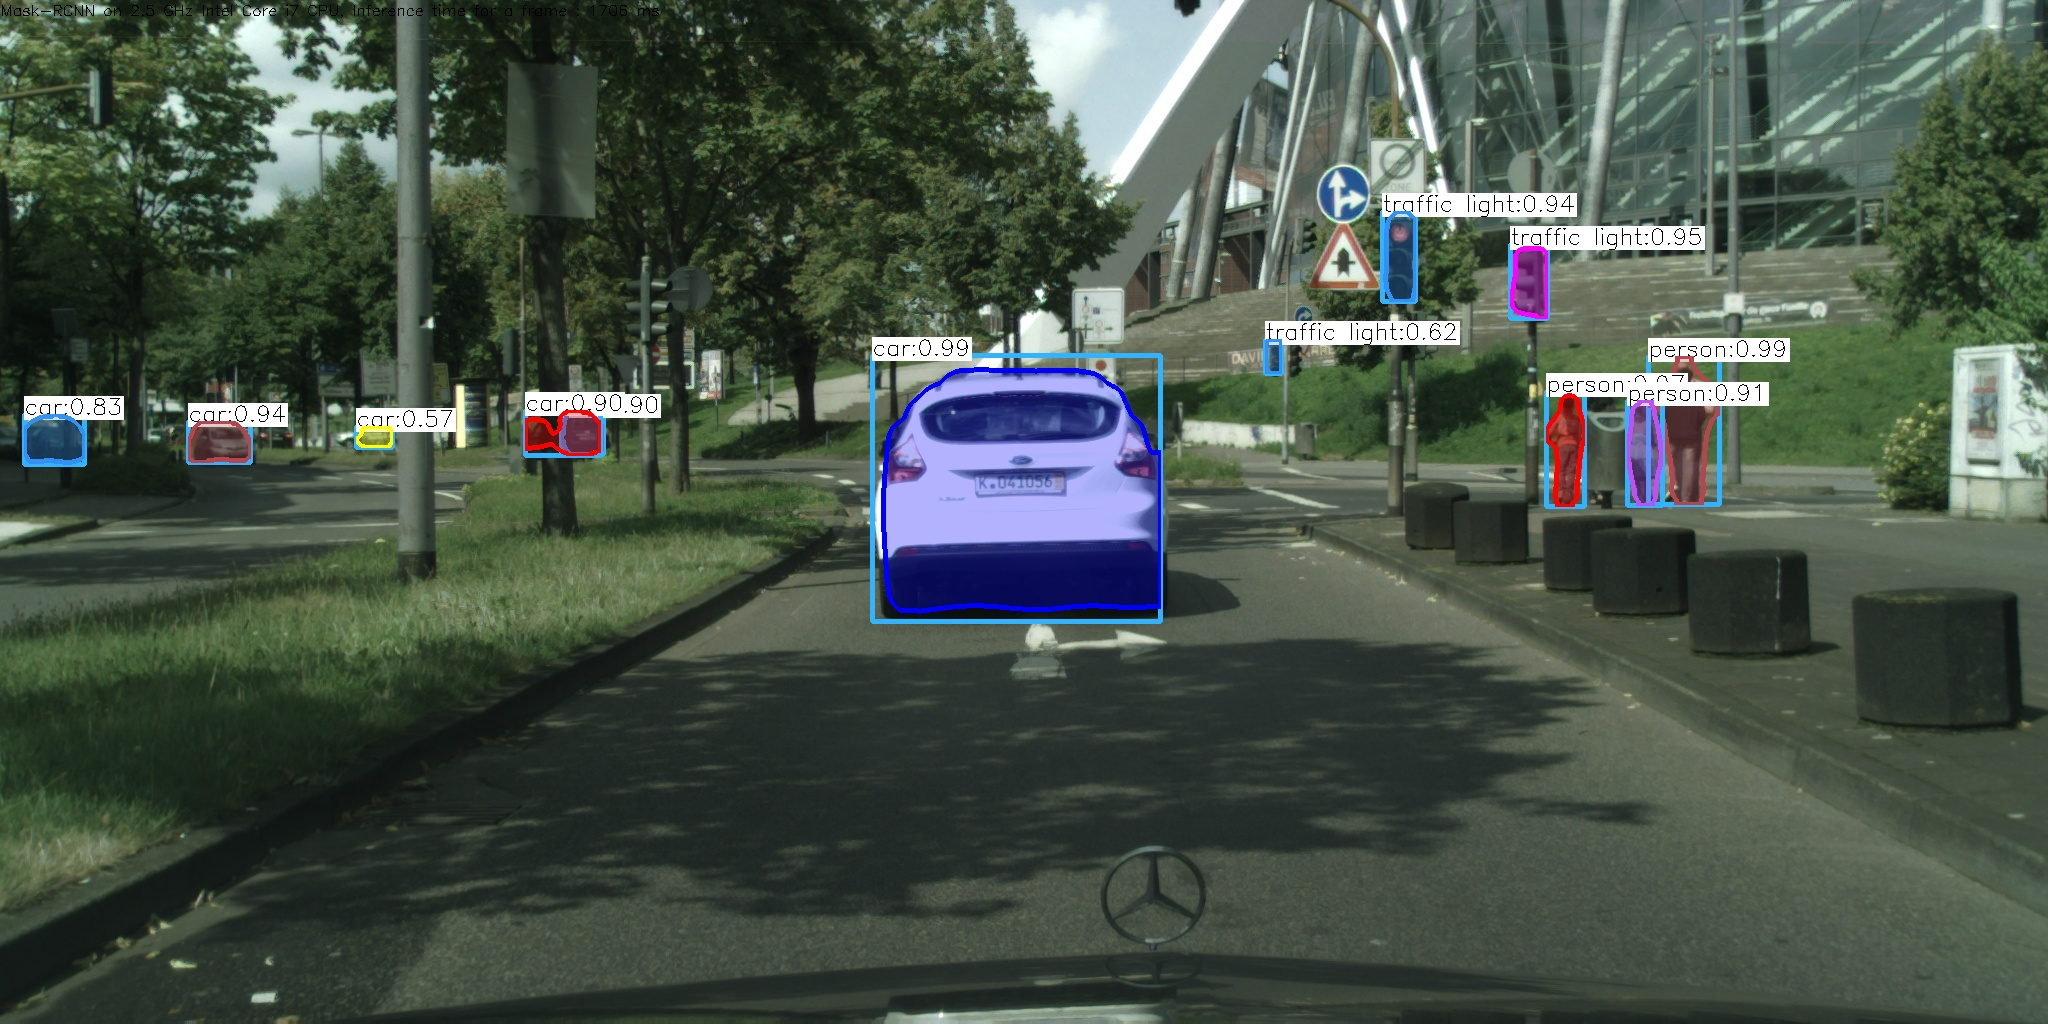
\includegraphics[width=2.7cm, height=2.7cm]{./figure/cologne_000011_000019_leftImg8bit_mask_rcnn_out_py.jpg}}\\ 
			\subfloat{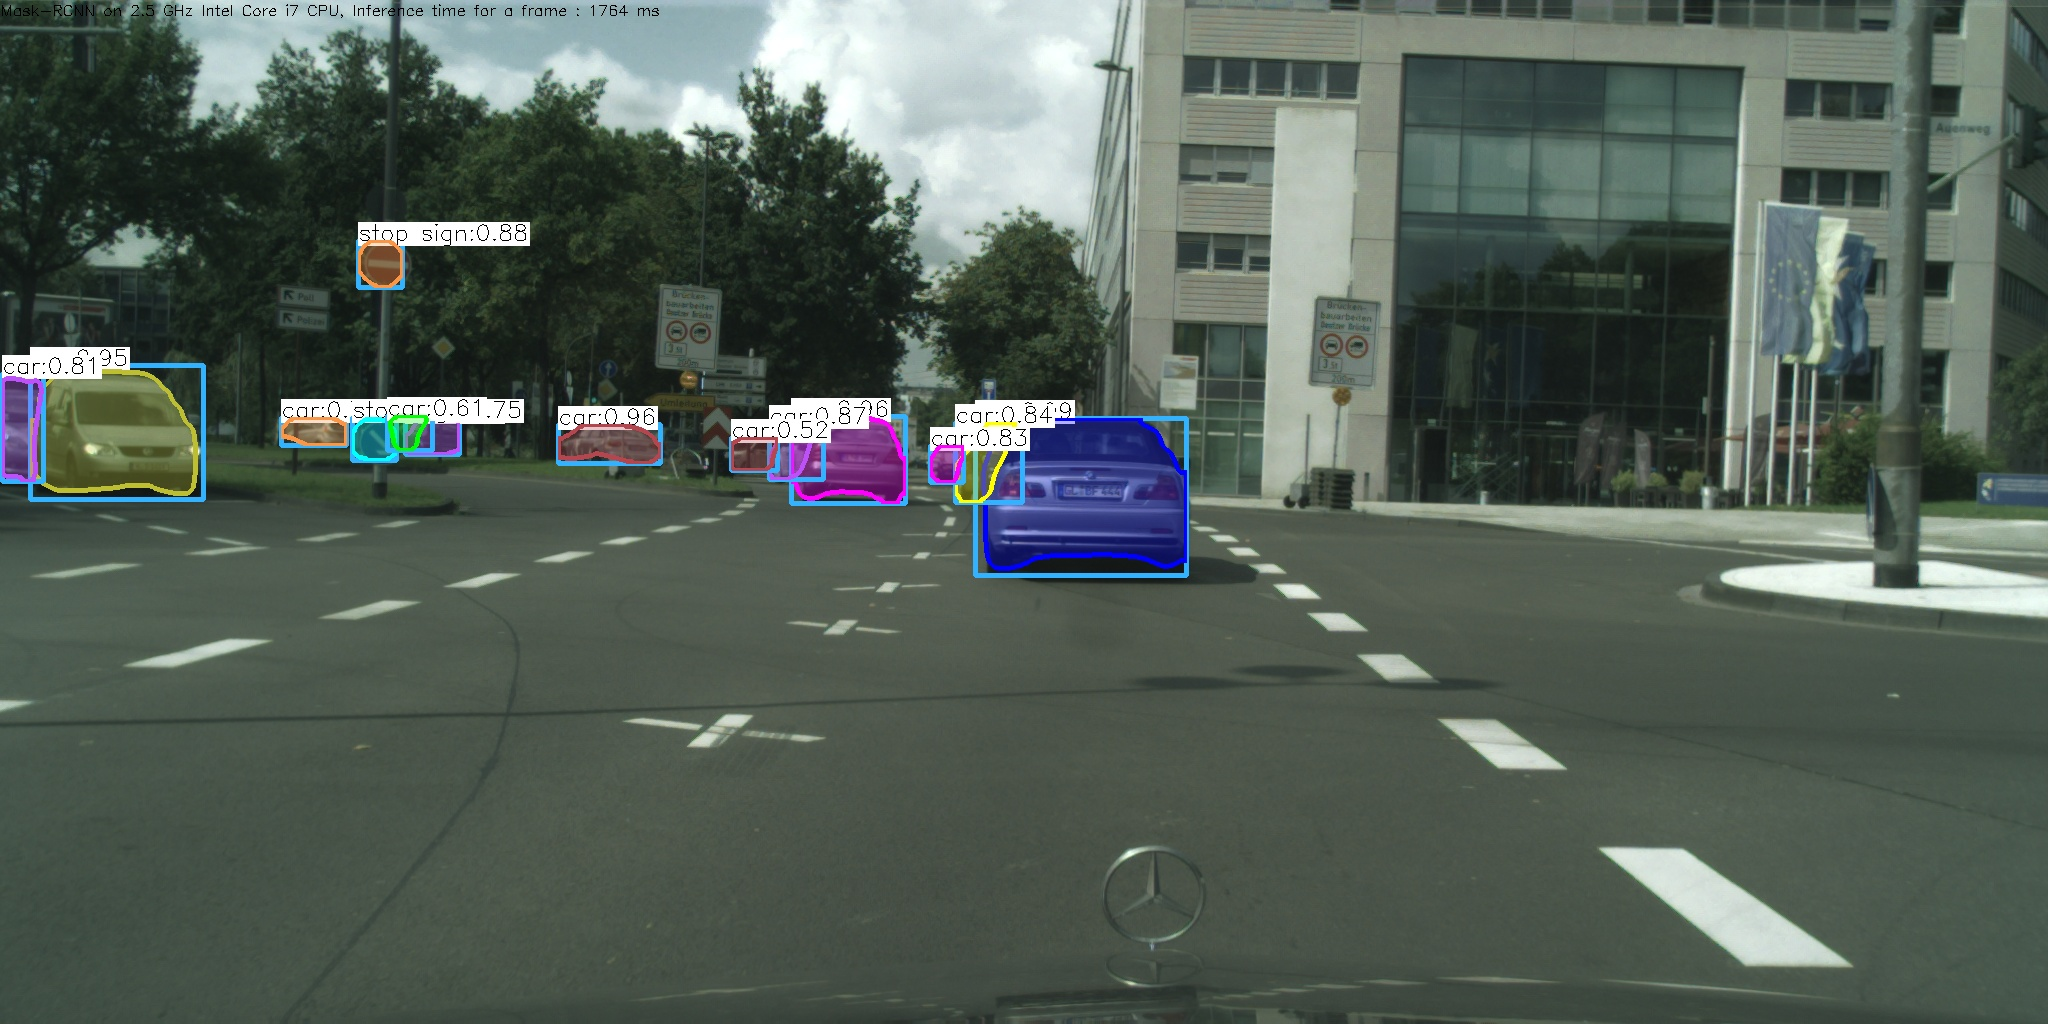
\includegraphics[width=2.7cm, height=2.7cm]{./figure/cologne_000013_000019_leftImg8bit_mask_rcnn_out_py.jpg}}\\
			\subfloat{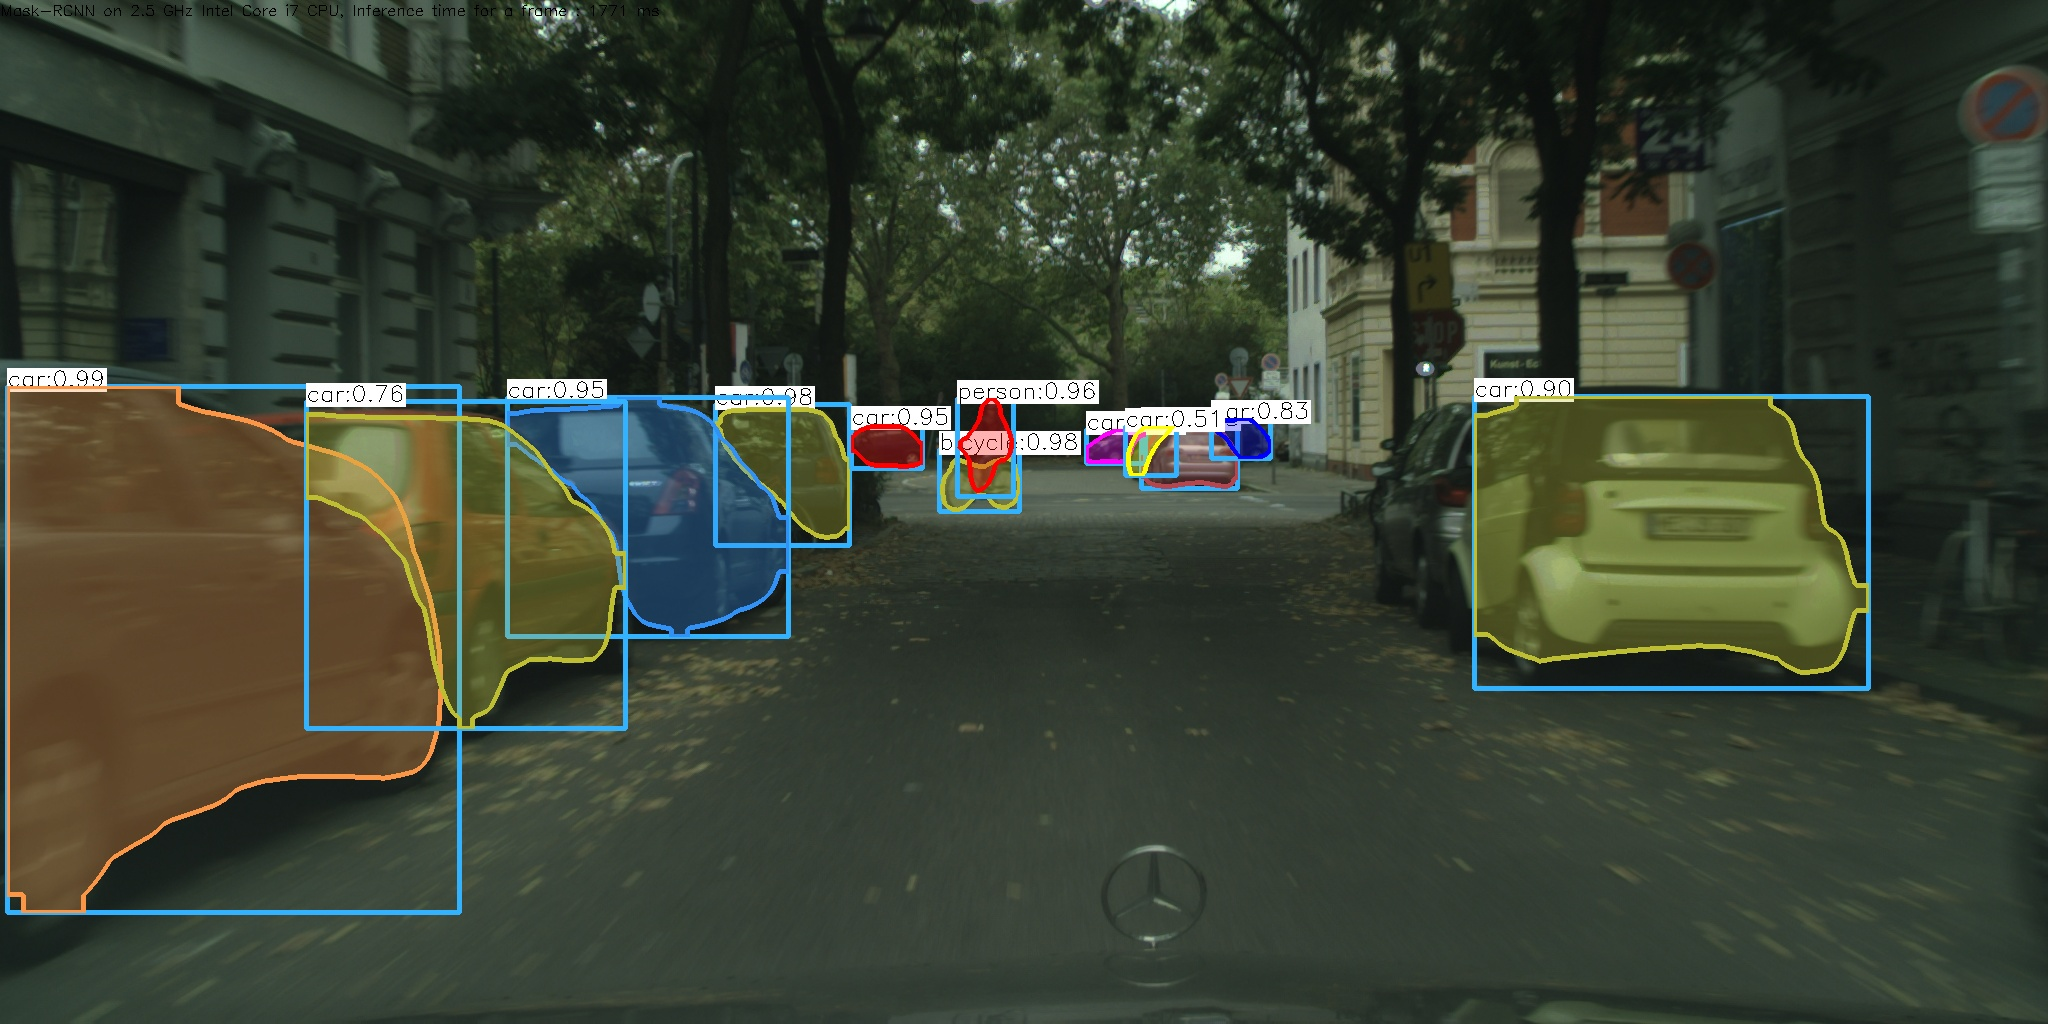
\includegraphics[width=2.7cm, height=2.7cm]{./figure/dusseldorf_000008_000019_leftImg8bit_mask_rcnn_out_py.jpg}}\\ 
			\subfloat{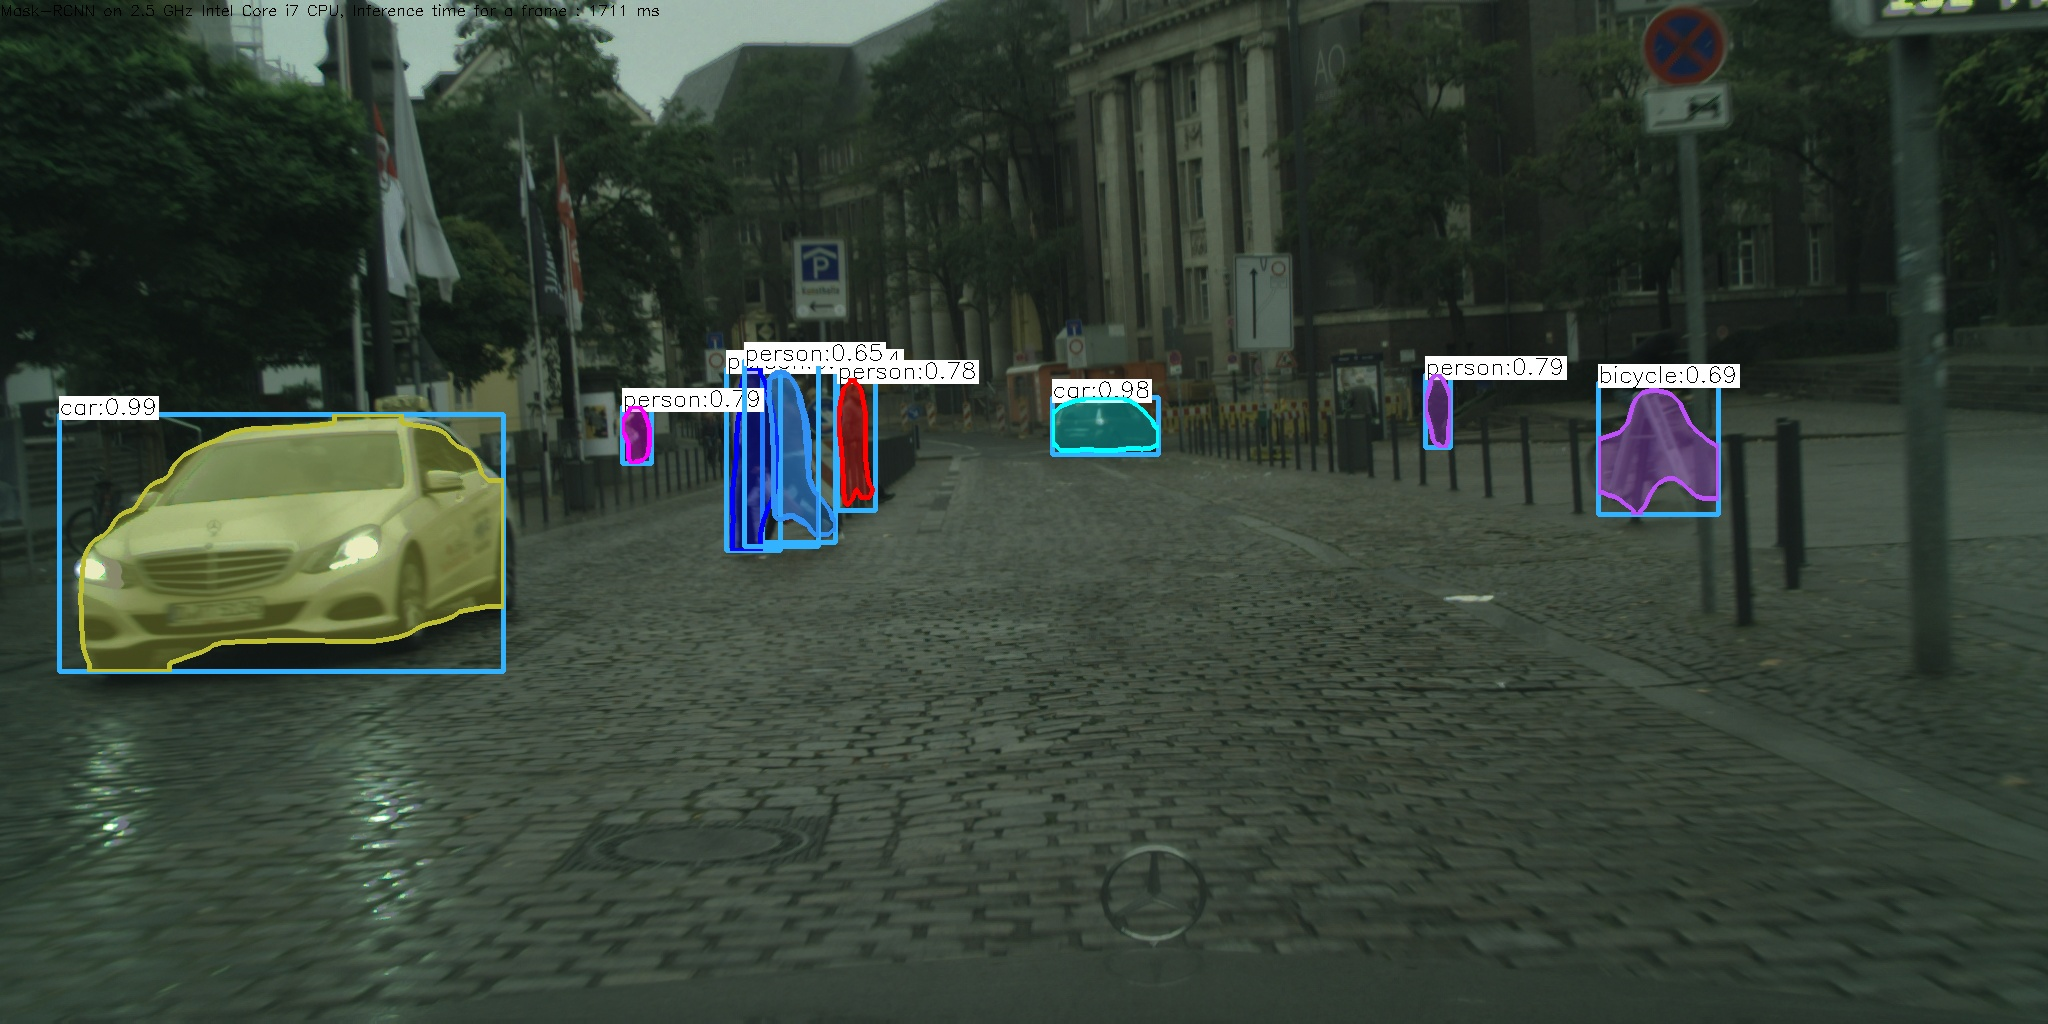
\includegraphics[width=2.7cm, height=2.7cm]{./figure/dusseldorf_000040_000019_leftImg8bit_mask_rcnn_out_py.jpg}}\\
			\subfloat{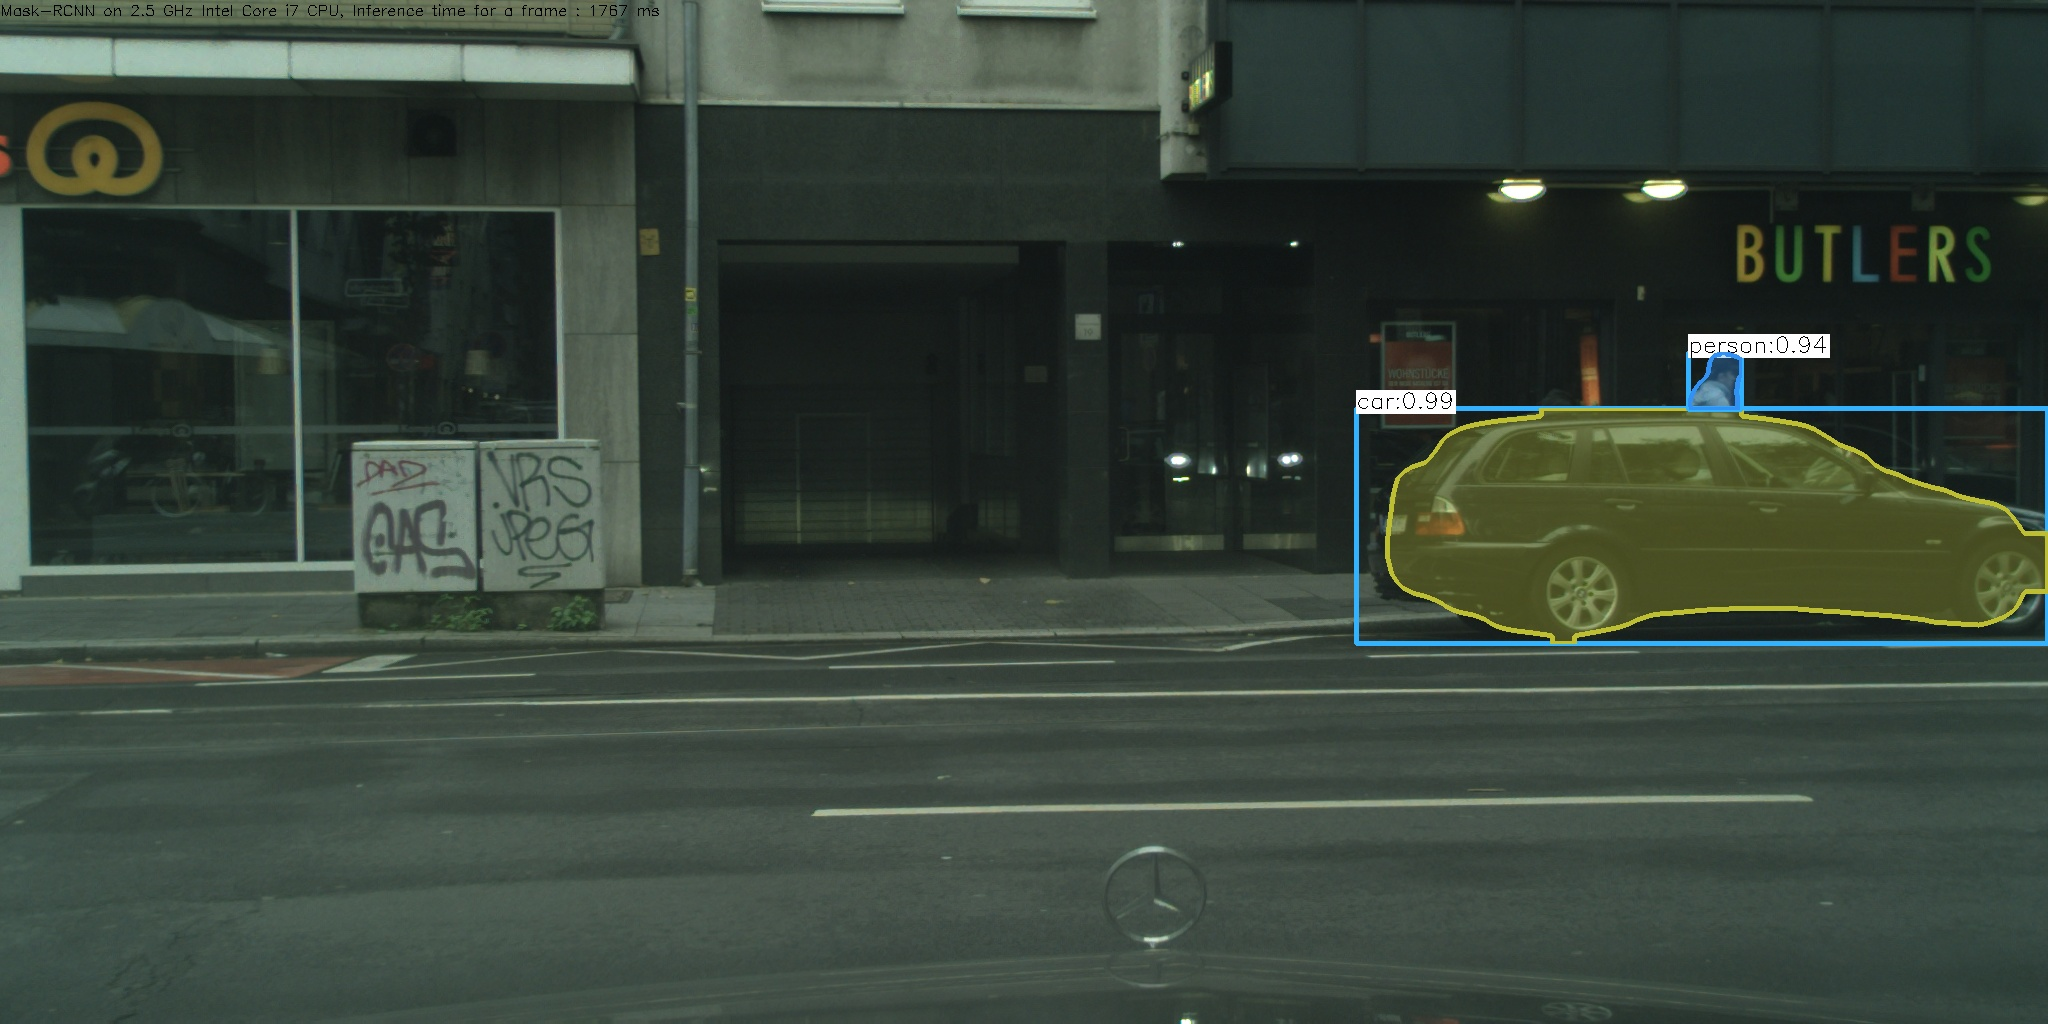
\includegraphics[width=2.7cm, height=2.7cm]{./figure/dusseldorf_000088_000019_leftImg8bit_mask_rcnn_out_py.jpg}}\\ 
			(b) detected cars \cite{rcnn} \\
		\end{tabular}
		&
		\begin{tabular}{cc}
			\subfloat{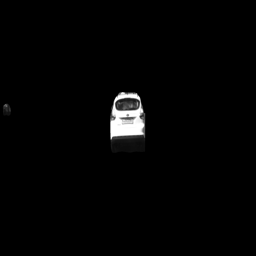
\includegraphics[width=2.7cm, height=2.7cm]{./figure/10_real_B}}\\ 
			\subfloat{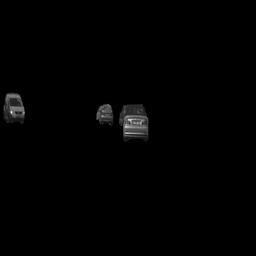
\includegraphics[width=2.7cm, height=2.7cm]{./figure/12_real_B}}\\
			\subfloat{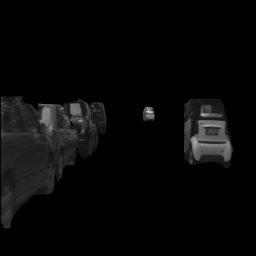
\includegraphics[width=2.7cm, height=2.7cm]{./figure/145_real_B}}\\ 
			\subfloat{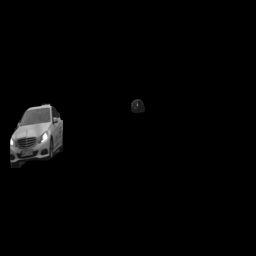
\includegraphics[width=2.7cm, height=2.7cm]{./figure/171_real_B}}\\
			\subfloat{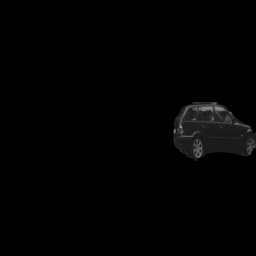
\includegraphics[width=2.7cm, height=2.7cm]{./figure/207_real_B}}\\ 
			(c) ground truth \\
		\end{tabular}
		&
		\begin{tabular}{cc}
			\subfloat{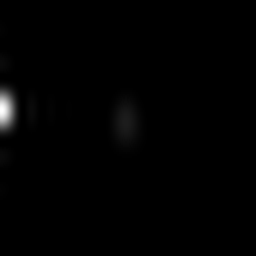
\includegraphics[width=2.7cm, height=2.7cm]{./figure/10_real_A}}\\ 
			\subfloat{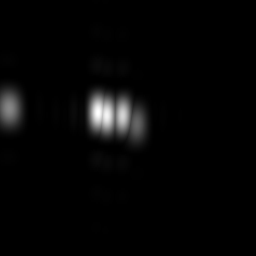
\includegraphics[width=2.7cm, height=2.7cm]{./figure/12_real_A}}\\
			\subfloat{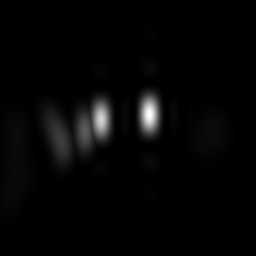
\includegraphics[width=2.7cm, height=2.7cm]{./figure/145_real_A}}\\ 
			\subfloat{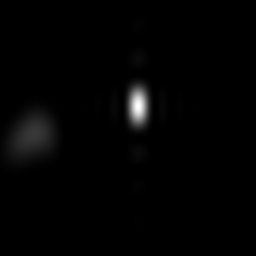
\includegraphics[width=2.7cm, height=2.7cm]{./figure/171_real_A}}\\
			\subfloat{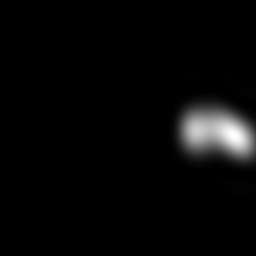
\includegraphics[width=2.7cm, height=2.7cm]{./figure/207_real_A}}\\ 
			(d) input heat-map \\
		\end{tabular}
		&
		\begin{tabular}{cc}
			\subfloat{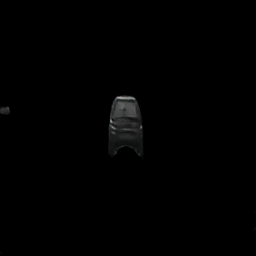
\includegraphics[width=2.7cm, height=2.7cm]{./figure/10_fake_B}}\\ 
			\subfloat{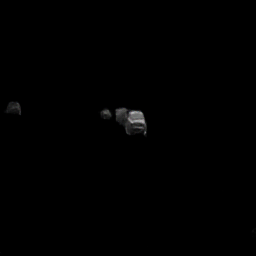
\includegraphics[width=2.7cm, height=2.7cm]{./figure/12_fake_B}}\\
			\subfloat{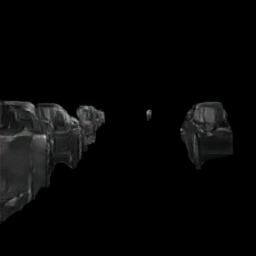
\includegraphics[width=2.7cm, height=2.7cm]{./figure/145_fake_B}}\\ 
			\subfloat{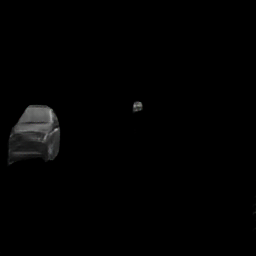
\includegraphics[width=2.7cm, height=2.7cm]{./figure/171_fake_B}}\\
			\subfloat{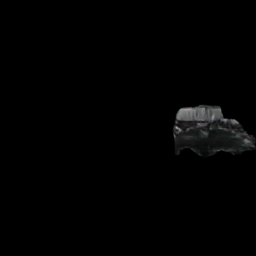
\includegraphics[width=2.7cm, height=2.7cm]{./figure/207_fake_B}}\\ 
			(e) generated image \\
		\end{tabular}
	\end{tabularx}	
	\caption{Some results from the second experiment. From top to bottom: 1) The car's boundary, shape and orientation has fully been recovered. The gray-scale colors do not much. However, colors are of little importance in our application. 2) The orientation of the middle car is reversed. As we shall see in the next section, 180 degrees of ambiguity can easily be fixed using the Doppler effect. 3) Although there is high reflection from the middle car, its boundary has correctly been identified as a small distant car. 4) Same as 3. Also the orientation of car on the side has been correctly estimated. 5) The generated image does not make sense. This is most likely because the sides of cars were rarely included in the training images provided to the network. }\label{fig2}
\end{figure*}
In the second experiment, as mentioned in the dataset section, we synthesized a more realistic dataset that is very similar to radar images. In most cases, the GAN was able to restore the boundaries and the orientation of the cars [figure]. It has also learned to identify the cars some of whose parts are blocked, either because they appear near the edge of image, or appear behind other cars.

As mentioned before, one significant problem with radar images is that some objects in appear to be much weaker or stronger in power than others, depending on their angle with the receiver mmWave antenna. The results from this experiment show that the GAN is able to learn this phenomenon and compensate for it. As a result, it is able to identify the cars, even if the reflection from them is weak [figure]. 
\subsection{}

\subsection{Dataset}
Training dataset 118 
Testing dataset 509
% Jayden

\subsection{Results}


\iffalse
We will conduct outdoor experiments on the top floor of the parking garage. Radar images (both 2D and 3D) will be collected with our custom-built Millimeter wave FMCW (Frequency Modulated Continuous Wave) radar system, operating around 60 GHz as shown in the figure above Both the radar transmitter and receiver antennas will be omni-directional. While the transmitter remains fixed, the receiver will move on a linear stage to synthesize a 1D or 2D antenna array to obtain the Direction of Arrival (DoA) measurement in a horizontal plane or the entire 3D space. We will first process raw radar data with fundamental radar signal processing algorithms, and filter out noise and unwanted interference to focus on only a few key features of the target. The target of interest can be either static or under motion. 

\subsection{Dataset Description}
The dataset we will create should include all significant features of a car. Therefore, we will place a car in a number of orientations in front of the radar, and try to filter out noise and interferences from other key points in pre-processing. We will also simulate the most likely relative positions and motions of the autonomous car with the radar system and other vehicles on the road, take a series of images as they move together.
\par We might have to face the problem of lack of accurate labels to our training set. One possible solution is to collect another set of reference data with cameras and train an additional neural network with well-developed vision models to label our radar images.

\begin{figure}
\centering
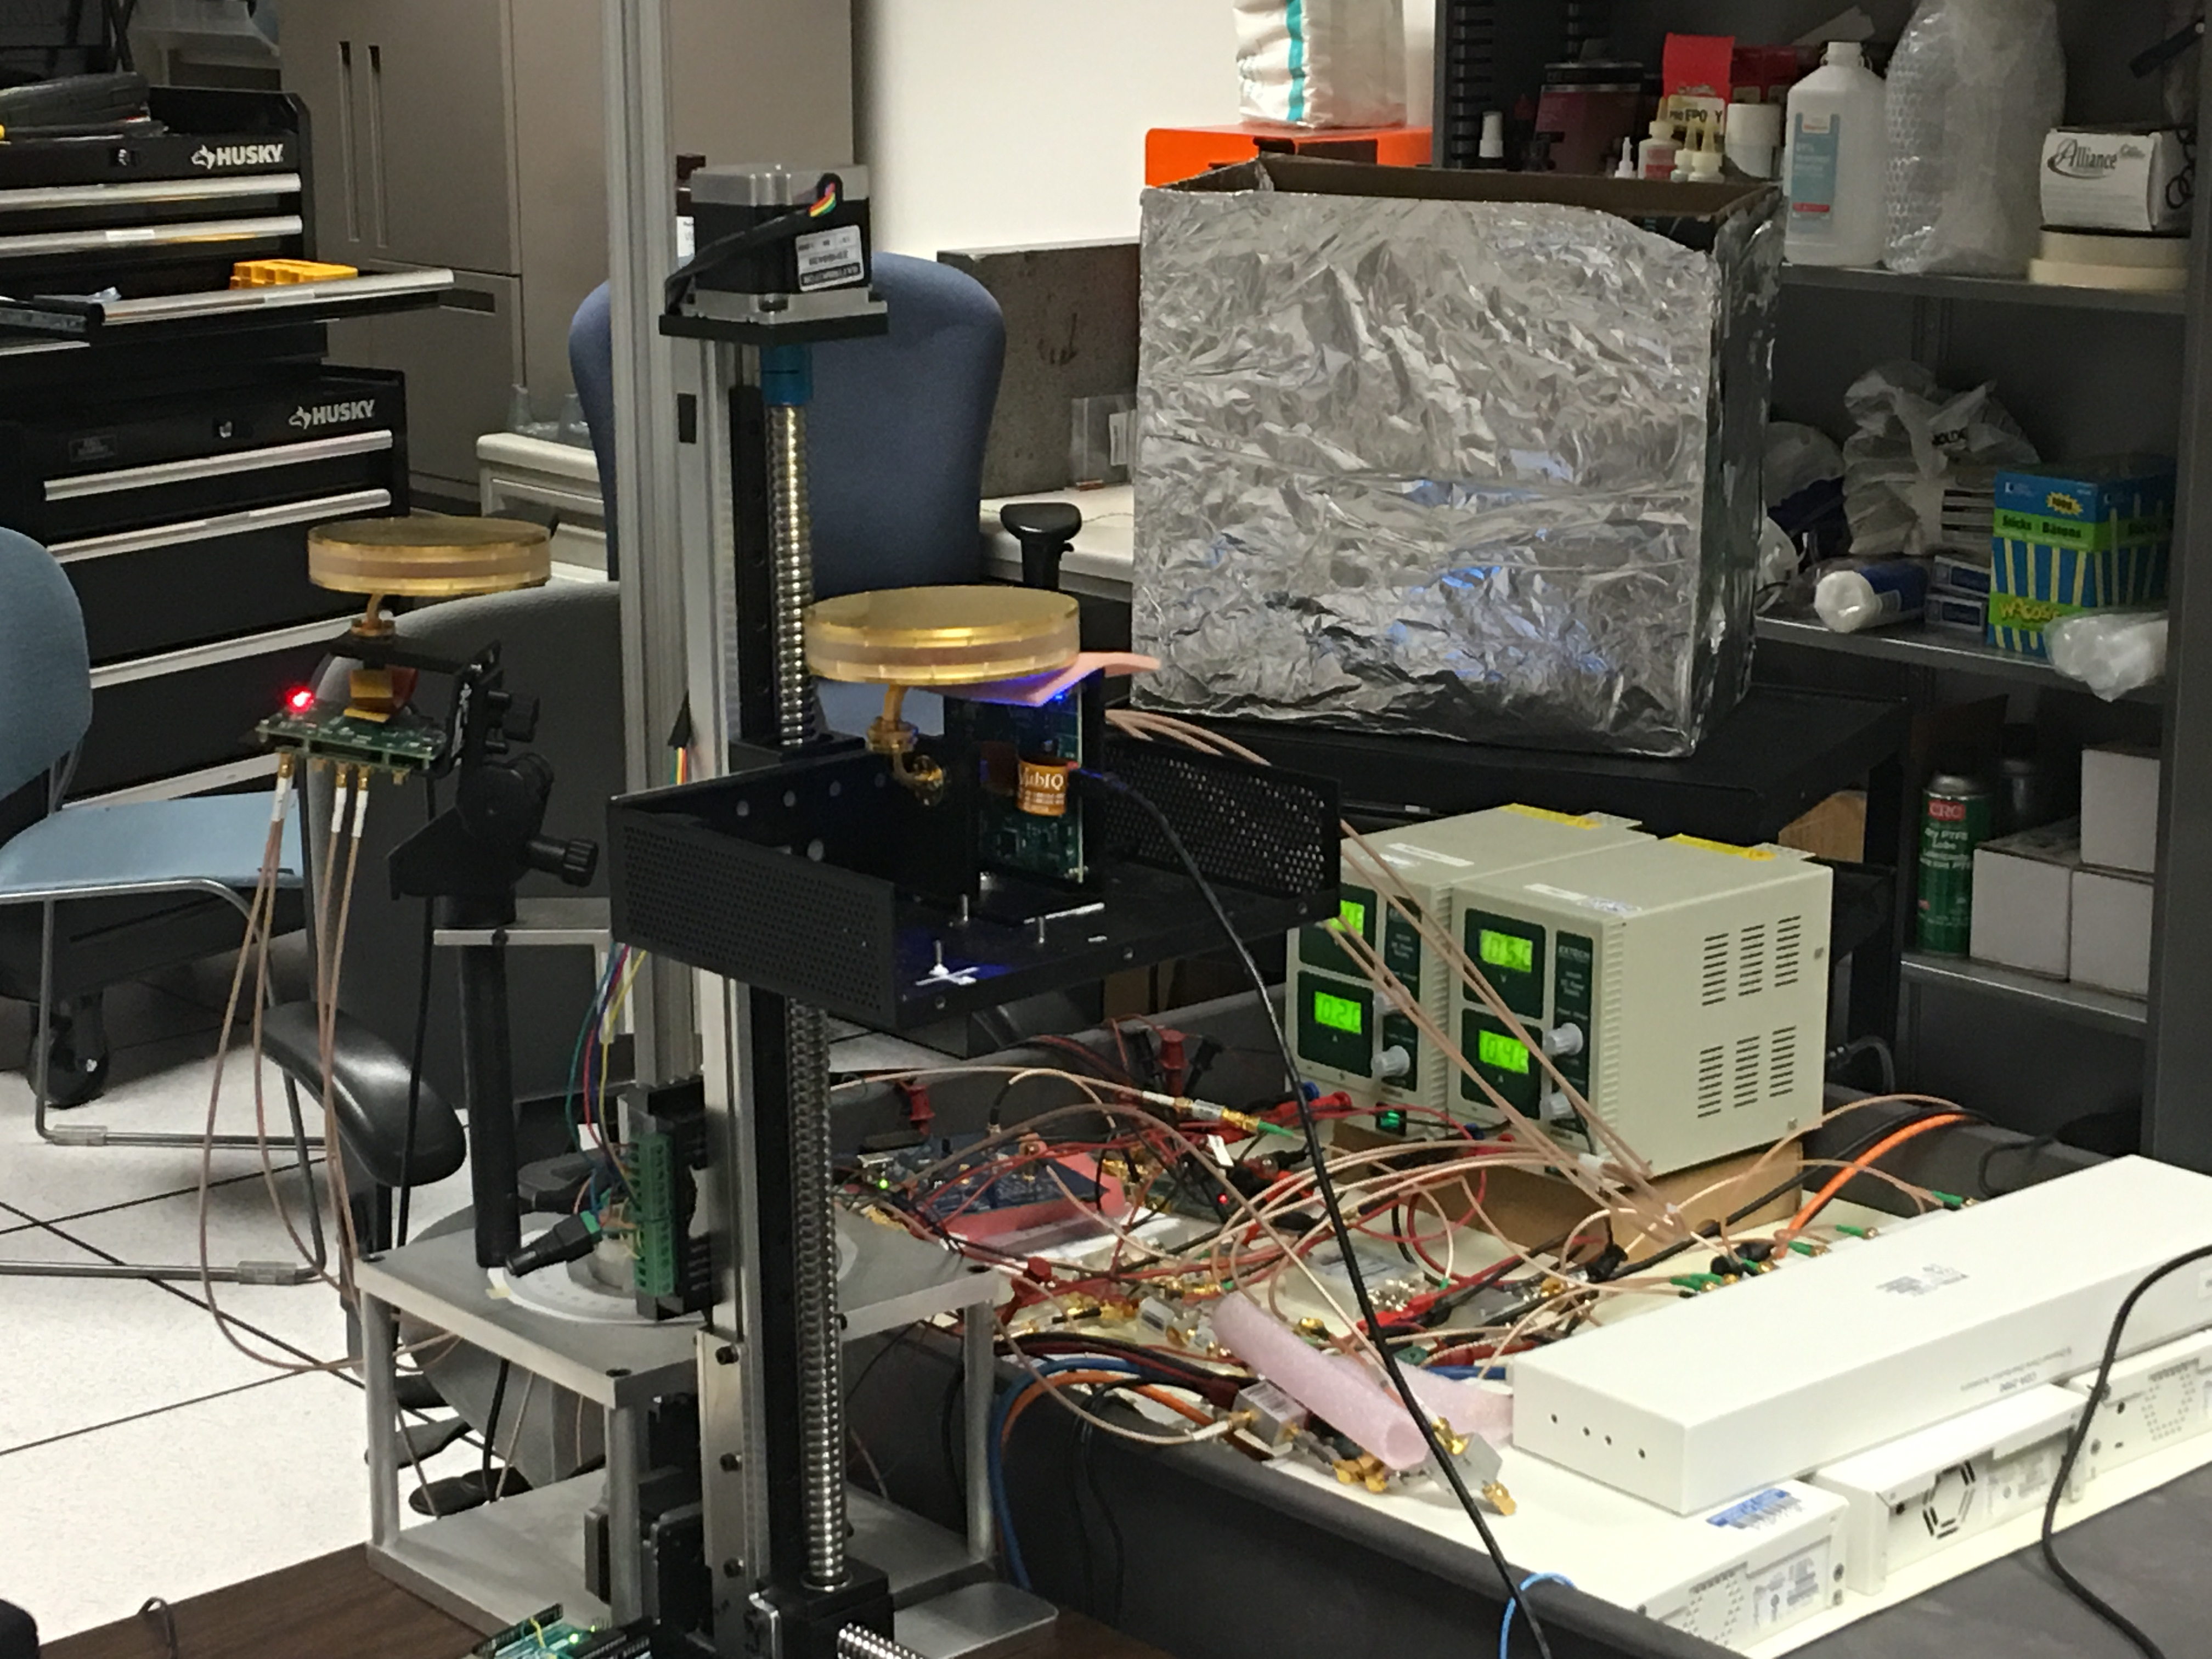
\includegraphics[width=8cm,height=6cm]{./figure/experiment_setup.jpg}
\caption{Custom-built 60 GHz mmWave radar imaging system}
\end{figure}

\fi
